\chapter{ DISCUSSÃO DE RESULTADOS} 


\par Neste capítulo são apresentados e discutidos os resultados obtidos na pesquisa realizada sobre o uso de testes automatizados no desenvolvimento de \textit{software} com o objetivo de destacar suas características, pontos principais e benefícios dessa abordagem.

\par Conforme citado em capítulos anteriores, o cenário utilizado para a demonstração de resultados foi um sistema web para a simulação de resultados de uma folha de pagamento. Através do uso do desenvolvimento orientado a testes (TDD), pôde-se perceber que há um grande benefício em se tratando de receber respostas de regressão, informações de problemas e falhas nas funcionalidades desenvolvidas para o sistema. 

\par Caso uma outra metodologia de desenvolvimento fosse adotada para o sistema que não o TDD, problemas seriam detectados tardiamente, visto que não haveria uma abordagem focada em testes tal como o TDD prega.





% \par Por isso o desenvolvimento orientado a teste (TDD) é muito mais rápido e eficaz.


\begin{figure}[!htb]
\centering
    \caption[TDD e Desenvolvimento Tradicional  ]{TDD e Desenvolvimento Tradicional.
     
     \raggedleft
     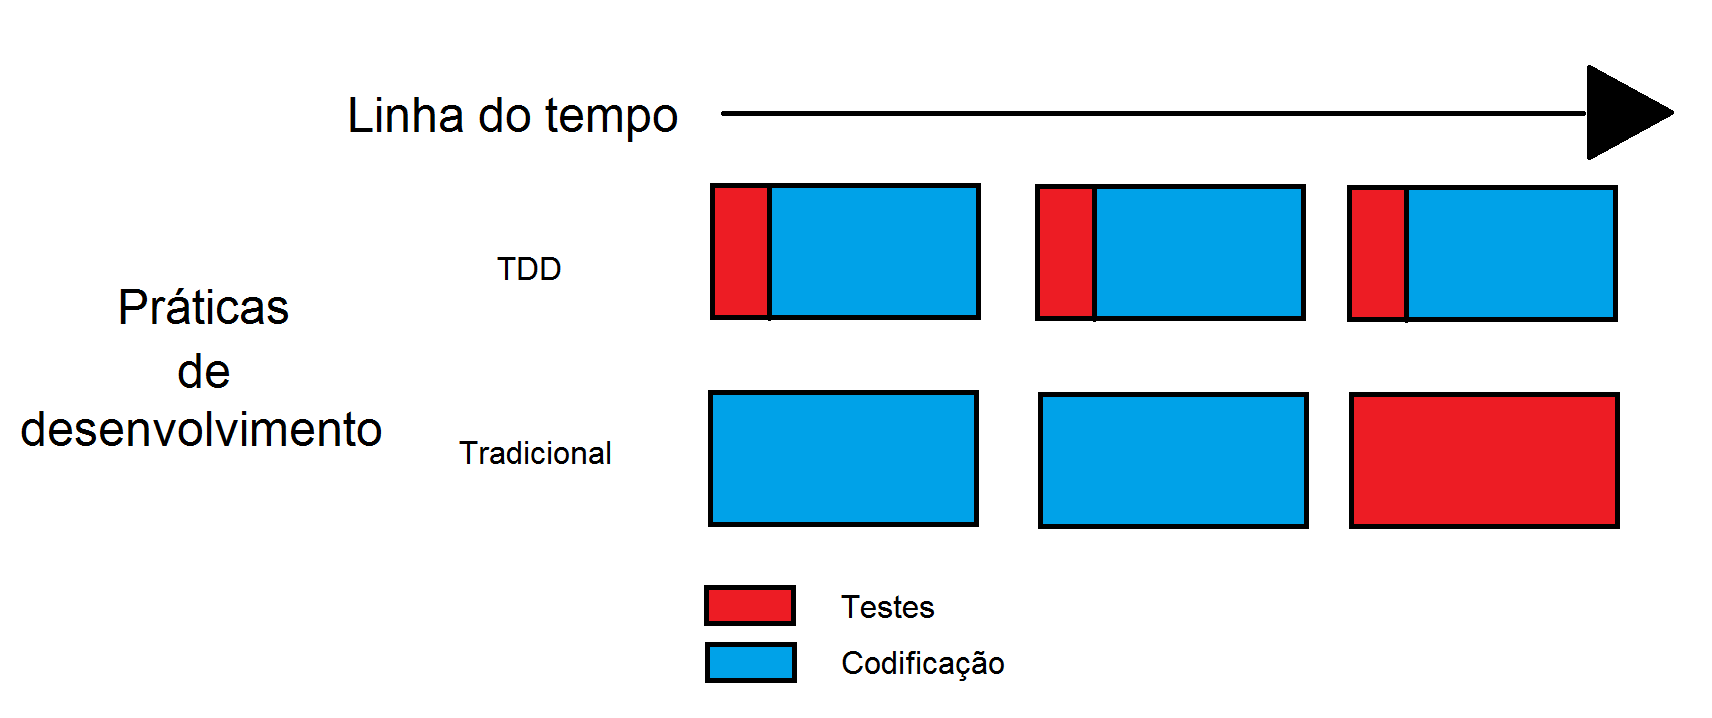
\includegraphics[scale=.35]{imagens/tdd.png}
     \centering
     \textbf{Fonte: } Elaborado pelos autores.}
     \label{fig:TDD e Desenvolvimento Tradicional}
\end{figure}


\par Vê-se, na Figura 50, como a metodologia TDD faz uso de testes: a cada porção de funcionalidade desenvolvida, há um ou mais testes automatizados desenvolvidos especialmente para garantir que aquele trecho irá funcionar conforme esperado e que todos os possíveis erros serão tratados. Com isso, pode-se prevenir erros futuros que já foram encontrados no momento do desenvolvimento do sistema. 

\par Já no segundo exemplo, vê-se que as funcionalidades são criadas e só então os testes são criados para estas. Muitas vezes, cenários deixam de ser cobertos pelos testes nessa metodologia, gerando uma porcentagem maior de falhas nos resultados finais.

\par Utilizando o desenvolvimento orientado a teste, obtém-se uma resposta rápida sobre se o módulo está funcionando corretamente, e assim, prevenir erros à frente. No exemplo da Figura 51, é demonstrado que os testes foram executados com sucesso, conforme o esperado.



\begin{figure}[!htb]
    \caption[Testes INSS Passando  ]{Testes INSS Passando.
     \centering
     
     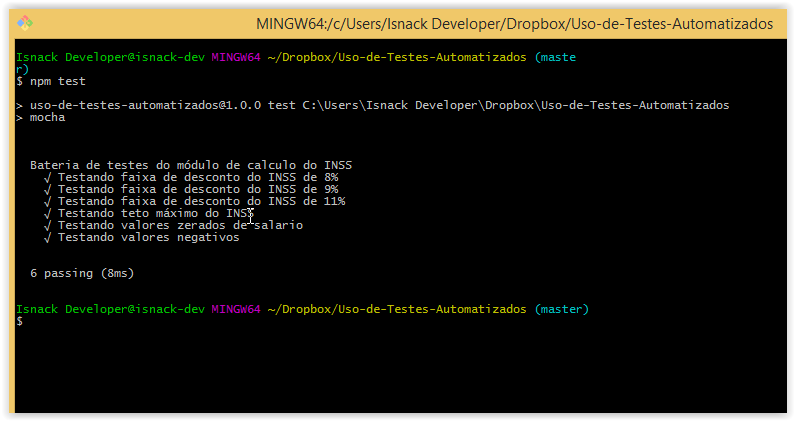
\includegraphics[width=12cm,height=8cm]{imagens/teste9.png}
     
     \textbf{Fonte: } Elaborado pelos autores.}
     \label{fig:testes INSS passando}
\end{figure}


\par A Figura 51 demonstra o uso de testes para cobrir várias possibilidades de uso do método o qual está sendo testado. No caso acima exemplificado, foi escolhida uma determinada porcentagem, a qual seria enviada para a funcionalidade que calcula o desconto do INSS (sobre o salário bruto do funcionário) para que esta retornasse um determinado resultado. Foi utilizado o \textit{framework} \textit{chai} e \textit{mocha} para facilitar a criação dos testes.




\par Este trabalho utilizou \textit{frameworks} para facilitar as realizações dos testes, criando vários cenários ou baterias de testes, sendo que, nesse cenário se específica o módulo que será testado. O Código 15 demonstra uma bateria de testes realizados neste trabalho

\clearpage
\newpage

    
\begin{comment}
    
\begin{figure}[!htb]
   \caption[Criação de todos os testes INSS ]{Criação de todos os teste INSS.
     \centering
     
     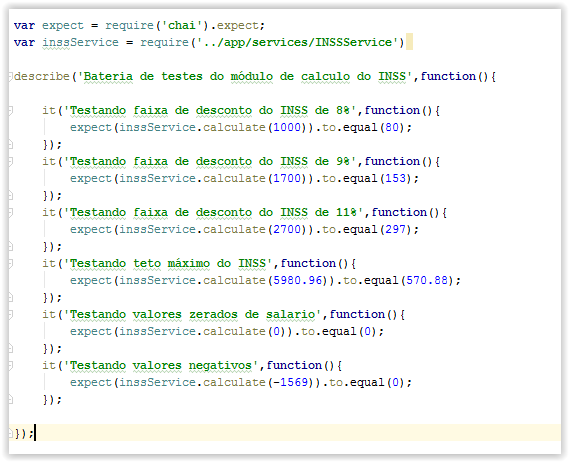
\includegraphics[width=12cm,height=6cm]{imagens/teste7.png}
     
     \textbf{Fonte: } Elaborado pelos autores.}
     \label{fig:todos teste inss}
\end{figure}

\end{comment}



\begin{lstlisting}[language=JavaScript, caption={[Criação de todos os testes INSS.]{Criação de todos os testes INSS.  \textbf{Fonte:} Elaborado pelos autores.}}]
var expect = require('chai').expect;
var inssService = require('../app/services/INSSService');

describe('Bateria de testes do módulo de calculo do INSS',function(){
    
    it('Testando faixa de desconto do INSS de 8%',function(){
        expect(inssService.calculate(1000)).to.equal(80);
    });
    it('Testando faixa de desconto do INSS de 9%',function(){
        expect(inssService.calculate(1700)).to.equal(153);
    });
    it('Testando faixa de desconto do INSS de 11%',function(){
        expect(inssService.calculate(2700)).to.equal(297);
    });
    it('Testando teto máximo do INSS',function(){
        expect(inssService.calculate(5980.96)).to.equal(570.88);
    });
    it('Testando valores zerados de salario',function(){
        expect(inssService.calculate(0)).to.equal(0);
    });
    it('Testando valores negativos',function(){
        expect(inssService.calculate(-1569)).to.equal(0);
    });
});

\end{lstlisting}



\par O Código 15, demonstra como os testes foram criados: um teste foi criado para cada possibilidade de desconto do INSS para um determinado salário bruto enviado para a funcionalidade. Os testes da Figura 51 finalizaram com sucesso, pois obedeciam o critério definido nos testes.

\par Comparado com os testes manuais os testes funcionais demonstraram um bom resultado na produtividade dos testes devido a sua automação para testar toda a funcionalidade da aplicação. Porém os testes funcionais tem um custo elevado devido a dificuldade do seu desenvolvimento em comparação ao desenvolvimento dos testes de unidade e integração.
 
 \par Um dos principais benefícios alcançados por esta pesquisa, foi a utilização da integração contínua (\textit{TravisCI}), sendo que, se a \textit{build} quebrar ou não, o \textit{TravisCI} encaminha um \textit{e-mail} avisando sobre a ocorrência. 
 
\par Uma grande vantagem de receber as notificações por \textit{e-mail}, é que hoje em dia todas as pessoas tem seu \textit{e-mail} sincronizado com seu \textit{smartphone}. Isso facilita a vida do desenvolvedor, pois assim que ocorre um evento, ele é notificado. Conforme mostra a Figura 52.
 
 
\begin{figure}[!htb]
    \caption[E-mail TravisCI envia ]{E-mail TravisCI envia.
     \centering
     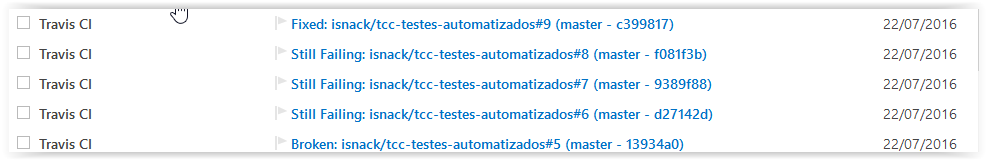
\includegraphics[width=14cm,height=3cm]{imagens/travis12.png}
     \textbf{Fonte: } Elaborado pelos autores.}
     \label{fig:e-mail TravisCI envia}
\end{figure}


\par Conforme a Figura 53, esse é o exemplo do \textit{e-mail} aberto logo após ser recebido e aberto na caixa de entrada. Sendo possível verificar o que está acontecendo no repositório.

\begin{figure}[!htb]
\centering
    \caption[E-mail aberto  ]{E-mail aberto.
    
     
     
     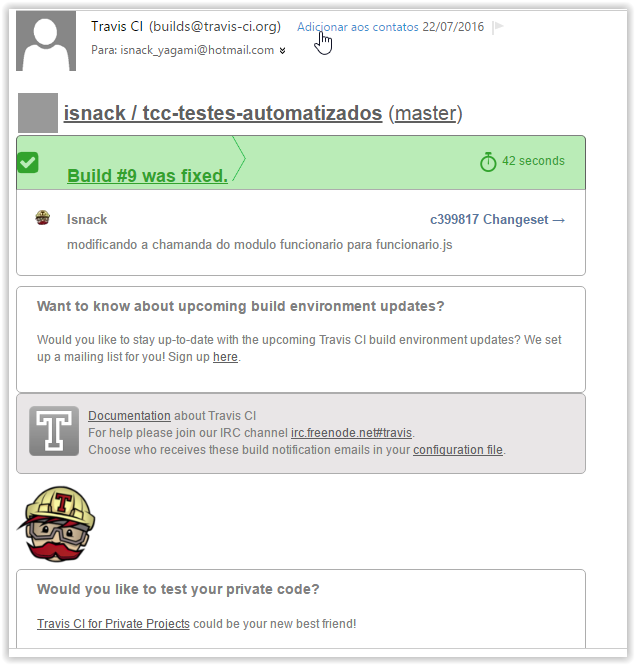
\includegraphics[scale=.75]{imagens/travis30.PNG}
     
     \textbf{Fonte: } Elaborado pelos autores.}
     \label{fig:e-mail aberto}
\end{figure}



\par Além de notificações via \textit{e-mail}, o \textit{TravisCI} também disponibiliza a integração na ocasião da integração de um \textit{pull request}; ou seja, qualquer contribuição é previamente testada pelo serviço antes que uma junção (\textit{merge}) seja efetivada com sucesso, a fim de evitar qualquer erro e/ou problema com o código atual. 

\par Se houver um problema com a integração, a ferramenta envia uma mensagem de \textit{e-mail} ao responsável para que o mesmo esteja ciente dos problemas que o código presente no \textit{pull request} podem potencialmente causar.

\par Há um \textit{check-list} com o resultado da integração: quais arquivos têm problema, quais foram responsáveis pela falha de determinados testes, dentre outros. Isso gera uma segurança e tranquilidade maior por parte dos desenvolvedores, pois podem previamente detectar problemas e erros antes que novas atualizações sejam atreladas ao produto atual.


\begin{figure}[!htb]
    \caption[Pull Request dando erro ]{Pull Request dando erro.
    
     \centering
     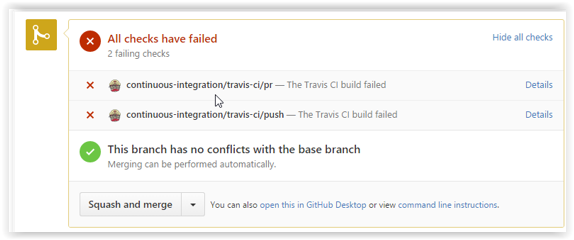
\includegraphics[width=12cm,height=6cm]{imagens/travis15.PNG}
     
     \textbf{Fonte: } Elaborado pelos autores.}
     \label{fig:Pull Request dando erro}
\end{figure}


\par A Figura 54 demonstrada é resultado de uma integração que apresenta problemas. Quando o \textit{pull request} foi feito, todos os interessados puderam realizar comentários e analisar as mudanças antes da mesma ser adicionada ao código de produção, a fim de garantir que potenciais problemas sejam evitados antes mesmo que as alterações sejam adicionadas ao produto.

\par Outro benefício foi a utilização do relatório de cobertura, o qual verifica a porcentagem de trechos de código que são verificados pelos testes e quais linhas de códigos ainda não são. Para os trechos que não estão sendo verificados, deve-se adicionar um grupo de testes para melhorar os índices de sucesso do relatório de cobertura.

\par Na Figura 55, as linhas em vermelho representam o número de linhas que faltam ser verificadas por testes automatizados e que necessitam de uma atenção especial.

\newpage

\begin{figure}[!htb]
    \caption[Relatório de Cobertura no qual tem partes que não estão cobertas ]{Relatório de Cobertura no qual tem partes que não estão cobertas.
    
     \centering
     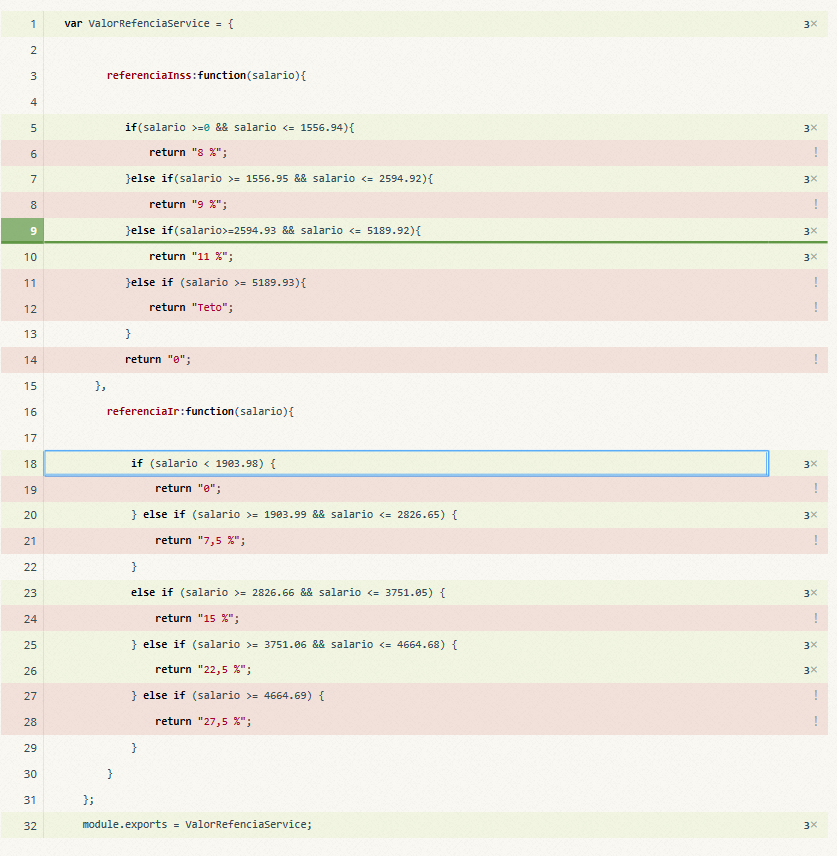
\includegraphics[width=15cm,height=15cm]{imagens/relatorio5.PNG}
     
     \textbf{Fonte: } Elaborado pelos autores.}
     \label{fig:Relatório de Cobertura no qual tem partes que não estão cobertas}
\end{figure}


\par Observa-se na Figura 55 que, após a análise de um desenvolvedor experiente, há a necessidade de uma melhoria no projeto, implementando e aprimorando testes nas unidades que ainda não estão cobertas e/ou não são verificadas. Com isso, o índice de cobertura do  projeto aumenta, melhorando os resultados posteriores ao buscar relatórios de testes automatizados.

\par Outra vantagem que o relatório de cobertura oferece é a integração com o \textit{coveralls.io} (ferramenta que proporciona o uso do relatório de cobertura online), o qual disponibiliza funcionalidades para gerenciar a porcentagem mínima aceitável de cobertura de testes. Caso esse índice não seja atingido, o código a ser integrado é considerado como falha. %Conforme mostra Figura 56.

\begin{figure}[!htb]
    \caption[Pull request dando erro no relatório de cobertura]{Pull request dando erro no relatório de cobertura.
    
     \centering
     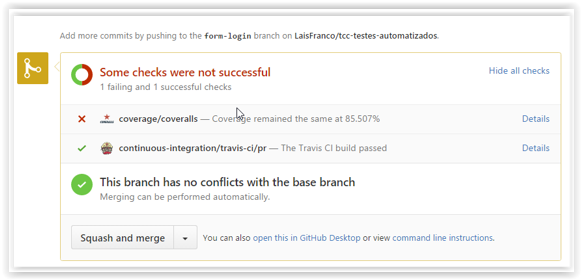
\includegraphics[scale=1.0]{imagens/discussao2.PNG}
     
     \textbf{Fonte: } Elaborado pelos autores.}
     \label{fig:Pull request dando erro no relatório de cobertura}
\end{figure}


\newpage
\par Como se pode observar na Figura 56, o \textit{coveralls.io} faz integração com o \textit{GitHub} e o \textit{TravisCI}. Toda vez que um \textit{pull request} é enviado, a ferramenta faz a análise do trecho de código enviado. Após a análise, um ícone em vermelho representa a porcentagem de código o qual não está propriamente verificado/coberto através de testes automatizados (o responsável pelo repositório ainda poderá realizar a mesclagem com o código principal; porém, um \textit{e-mail} será enviado aos interessados alertando a porcentagem de cobertura do código para aquele \textit{pull request} enviado).

\par Conclui-se que o uso de ferramentas de testes automatizados é benéfico aos desenvolvedores de \textit{software}, auxiliando-os a entregar sistemas com o menor índice possível de falhas e erros (\textit{bugs}), os quais são detectados com antecedência através do uso dessas ferramentas. A satisfação do cliente se torna maior ao usar um \textit{software} com o mínimo de erros possíveis.




\begin{comment}
    

\par A figura acima mostra que foram testadas várias possibilidades de testes, sendo que em cada possibilidade executada especificou-se uma determinada porcentagem, que se refere ao desconto do INSS sobre o salário bruto do funcionário.


\par A figura acima demonstra uma maneira simplificada do que foi falado acima, sendo que o vermelho representa os testes e o azul o desenvolvimento do sistema.
\par O objetivo da pesquisa foi demonstrar através da criação de uma folha de pagamento web, a utilização dos testes automatizados.   


\par No processo de desenvolvimento orientado a testes (TDD), percebe-se que ao criar os testes e executá-los, há uma resposta rápida se o método está funcionando corretamente.


\par Está resposta rápida não é obtida com sucesso quando usado os testes manuais ou desenvolvimento tradicional, pois nesse processo, se desenvolve boa parte do sistema antes de aplicar os testes e a verificação se está funcionando corretamente ou não.


\par Se usar os testes manuais ou o desenvolvimento tradicional, que nada mais é do que desenvolver boa parte do sistema para depois aplicar os testes e assim verificar se está tudo funcionando corretamente, as repostas obtidas iram demorar um pouco mais, do que usar o desenvolvimento orientado a testes.
\par Entre os principais benefícios alcançados por esta pesquisa, pode-se afirmar que o \textit{pull-request} desempenho um grande 



\par Neste capítulo tem por finalidade descrever os resultados obtidos nesta pesquisa através de uma explicação teórico-prática. 

\par O presente trabalho teve por objetivos desenvolver testes automatizados, mostrando assim que quando mais teste são feitos, menor e o índice do \textit(software) apresentar falhas, sendo possível ter um índice de cobertura do sistema maior.

\par o objetivo da pesquisa foi demonstrar como o uso de testes automatizados detém a melhorar significativamente o desenvolvimento de uma folha de pagamento web.

 \end{comment}





